\documentclass[]{article}

\usepackage[UTF8]{ctex}
\usepackage[a4paper,scale=.7]{geometry}
\usepackage{amsmath,amsfonts,mathrsfs,amssymb,ntheorem,extarrows,graphicx,enumerate,braket,mathtools,xcolor,listings,syntonly,multicol}
%\usepackage{showlabels}


%\numberwithin{equation}{section}

\newcommand*\diff{\mathop{}\!\mathrm{d}}
\newcommand*\Diff[1]{\mathop{}\!\mathrm{d^#1}}
\newcommand*\bd{\mathop{}\!\text{\dj}}

\newcommand\der[1]{\frac{\diff}{\diff #1}}
\newcommand*\Der[2]{\frac{\diff #1}{\diff #2}}
\newcommand\nder[2]{\frac{{\diff}^#1}{{\diff #2}^#1}}
\newcommand*\nDer[3]{\frac{{\diff}^#1 #2}{{\diff #3}^#1}}
\newcommand\parder[1]{\frac{\partial}{\partial #1}}
\newcommand*\parDer[2]{\frac{\partial #1}{\partial #2}}
\newcommand\nparder[2]{\frac{\partial^#1}{{\partial #2}^#1}}
\newcommand*\nparDer[3]{\frac{\partial^#1#2}{{\partial #3}^#1}}%定义导数的快捷输入

\renewcommand*\geq\geqslant
\renewcommand*\leq\leqslant
\renewcommand*\ge\geqslant
\renewcommand*\le\leqslant

\renewcommand*\phi\varphi
\renewcommand*\epsilon\varepsilon
\renewcommand*\deg{^\circ}

\renewcommand*{\(}{\left(}
\renewcommand*{\)}{\right)}

\newcommand\equs[1]{\left\{\, #1\right.}

\newcommand*\ee{\mathrm{e}}
\newcommand*\ii{\mathrm{i}}
\newcommand*\vXi{\varXi}

\newcommand\vcbd[1]{\boldsymbol{#1}}

\newcommand*\unit[1]{\,\mathrm{#1}}
\newcommand*\e[1]{\times 10^{#1}}
\newcommand*\myemph[2]{\emph{#1}(\emph{#2})}

\newcommand*\taghere{\refstepcounter{equation}\tag{\theequation}}

\newcommand*\xde{Schrödinger}
\newcommand*\xdefc{\xde 方程}
\newcommand*\dbly{de Broglie}
\newcommand\expe[1]{\left\langle #1 \right\rangle}

\newcommand*\operaise{\hat{a}_+}
\newcommand*\opelower{\hat{a}_-}
\newcommand*\opeladder{\hat{a}_\pm}
\newcommand*\commutator[2]{\left[\hat{#1},\hat{#2}\right]}
\newcommand*\ope[1]{\hat{#1}}
\newcommand*\opeadj[1]{\hat{#1}^\dag}

\newcommand*\ex{\vcbd{e_x}}
\newcommand*\ey{\vcbd{e_y}}
\newcommand*\ez{\vcbd{e_z}}
\newcommand*\er{\vcbd{e_r}}
\newcommand*\etheta{\vcbd{e_\theta}}
\newcommand*\ephi{\vcbd{e_\phi}}

\newcommand*\hilbert{\mathcal{H}}

\newtheorem*{props}{命题}
{
	\theorembodyfont{\normalfont}
	\newtheorem{exam}{例}
}
{
\theoremstyle{plain}
\newtheorem{exer}{}
}
{
\theoremstyle{nonumberplain}
\theorembodyfont{\normalfont}
\newtheorem{ans}{解:}
}
{
	\theoremstyle{nonumberplain}
	\theorembodyfont{\normalfont}
	\newtheorem{proof}{证:}
}

\newenvironment{Figure}
{\par\medskip\noindent\minipage{\linewidth}}
{\endminipage\par\medskip}

\lstset{
	basicstyle          =   \sffamily,          % 基本代码风格
	keywordstyle        =   \bfseries,          % 关键字风格
	flexiblecolumns,                % 别问为什么,加上这个
	numbers             =   left,   % 行号的位置在左边
	showspaces          =   false,  % 是否显示空格,显示了有点乱,所以不现实了
	numberstyle         =   \ttfamily,    % 行号的样式,小五号,tt等宽字体
	showstringspaces    =   false,
	frame               =   lrtb,   % 显示边框
	breaklines			=	true,
	backgroundcolor=\color{black!5},
}%定义代码抄录环境

\DeclareMathOperator{\li}{Li}

\title{统计物理随笔}
\author{龍翔九州}
\date{\today}

\begin{document}
	\maketitle
	\section{理想气体的统计分布}
	这几章主要考虑玻色气体和费米气体的统计性质。在自由气体近似下构成气体的玻色子 及费米子的能级与经典理想气体并没有什么区别,它们的统计特性主要来自于多个玻色子 或费米子带来的全同粒子效应以及泡利不相容原理。我们首先考虑单个粒子的能级,将粒子近似为在体积$ V $的范围内运动,能级近似能级视为准连续是粒子的德布罗意波长,那么粒子的能级$E=p^2/2m$. 粒子在能级$ E $附近的态密度$ g(E) $为\footnote{\eqref{first}式中分子的$4\pi p^2\diff p$代表$ \vcbd{p}- $空间中能量为$ E $至$ E+\diff E $的区域所占据的球壳体积,自然有$ E=p^2/2m $及$ \diff E=p\diff p/m $。分母的$ (2\pi\hbar)^3/V $代表每个$ \vcbd{p} $态所占据的体积,两个体积相除就得到了$ E $至$ E+\diff E $范围内的量子态数目。}
	\[\label{first}g(E)\diff E=\frac{4\pi p^2\diff p}{(2\pi\hbar)^2/V}\times g=g\frac{V}{\sqrt{2}\pi^2\hbar^3}m^{\frac 32}\sqrt E\diff E\taghere\]
	常数$ g $代表由于粒子自旋引入的简并度。式\eqref{first}即
	\[\label{DensityOfState}g(E)=g\frac{m^{\frac 32}V}{\sqrt{2}\pi^2\hbar^3}\sqrt E\taghere\]
	若能知道粒子在能级上的分布$ f(E) $, 即能级$ E $上量子态被粒子实际占据的比例,就能得到气体的热力学性质,例如
	\begin{subequations}\label{StatisticalQuantity}
		\begin{align}
			\label{3a}N&=\int_0^\infty f(E)g(E)\diff E\\
			U&=\int_0^\infty Ef(E)g(E)\diff E
		\end{align}
	\end{subequations}
	\begin{subequations}\label{Distribution}
		对于玻色气体,其分布为
		\[\label{BoseDistribution}f_{\text{Bose}}(E)=\frac 1{\ee^{\frac{E-\mu}{kT}}-1}\taghere\]
		对于费米气体,其分布为
		\[\label{FermiDistribution}f_{\text{Fermi}}(E)=\frac{1}{\ee^{\frac{E-\mu}{kT}}+1}\taghere\]
	\end{subequations}
	式\eqref{Distribution}的推导教材上已经详细写出,不再重复。
	\section{玻色气体}\label{sec:2}
	现在理想气体的统计理论框架已经搭好了,只要把式\eqref{DensityOfState}和\eqref{BoseDistribution}哐哐往\eqref{StatisticalQuantity}里代就完成了……本应如此,我们先实际代入一下。玻色子自旋假设为0,这样就没有自旋带来的简并:
	\[\label{5}N=\frac{m^{\frac 32}V}{\sqrt{2}\pi^2\hbar^3}\int_0^\infty\frac{\sqrt{E}\diff E}{\ee^{(E-\mu)/kT}-1}\taghere\]
	作换元$ E\to kTx $,引入参数$ z=\ee^{\mu/kT} $,那么
	\[\label{6}N=\frac{m^{\frac 32}V}{\sqrt{2}\pi^2\hbar^3}(kT)^{\frac 32}\int_0^\infty\frac{\sqrt{x}\diff x}{z^{-1}\ee^x-1}=\frac{m^{\frac 32}V}{\sqrt{2}\pi^2\hbar^3}(kT)^{\frac 32}\cdot\frac{\sqrt\pi}{2}h_{\frac 32}(z)\taghere\]
	其中
	\[\label{int}h_\nu(z):=\frac 1{\Gamma(\nu)}\int_0^{\infty}\frac{x^{\nu-1}}{z^{-1}\ee^x-1}\diff x\taghere\]
	$ h_\nu(z) $并不是初等函数,但是可以表达为级数
	\[\label{series}h_\nu(z)=\sum_{n=1}^\infty\frac{z^n}{n^\nu}=\li_\nu(z)\taghere\]
	通过级数表达式我们发现$ h_\nu(z) $就是多对数函数$ \li_s(z) $。不过我们不太需要这么花里胡哨的名字,就还是叫它$ h_\nu(z) $好了。我们把$ h_\nu(z) $画出来,看看它是什么样的:
	\begin{figure}[h]
		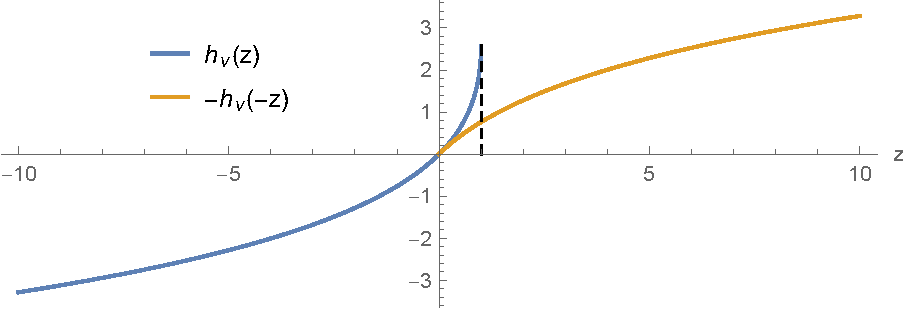
\includegraphics[width=\linewidth]{fig1}\label{fig1}
	\end{figure}
	蓝线就是我们要用到的$ h_\nu(z) $,黄线为讨论费米分布时需要用到的另一个函数$ g_\nu(z) $, 这里一并画出。
	
	我们发现$ h_\nu(z) $只有在$ z\le 1 $的时候有定义,在$ z>1 $的时候不仅级数\eqref{series}发散至$ \infty $,积分\eqref{int}本身也发散。并且按照级数\eqref{series}有
	\[h_\nu(1)=\sum_{n=1}^{\infty}\frac{1}{n^\nu}=\zeta(\nu)\taghere\]
	$ \zeta(\nu) $是另一个特殊函数,没别的了。对于玻色子来说我们只需要关心$ z>0 $的情况,毕竟$ \ee^{\mu/kT}>0 $.但是对于费米子我们会涉及到另一个积分
	\[g_\nu(z):=\frac{1}{\Gamma(\nu)}\int_0^\infty\frac{x^{\nu-1}}{z^{-1}\ee^x-1}\diff x=-h_\nu(-z)\taghere\]
	相当于把$ h_\nu(z) $在第四象限的部分旋转到第一象限,在上图里我们一并画了出来。
	
	把式\eqref{6}变形有
	\[\label{61}h_{\frac 32}(z)=\left(\frac{2\pi\hbar^2}{mkT}\right)^{\frac 32}\frac NV\taghere\]
	式\eqref{61}相当于一个方程,对一个给定温度$ T $的理想玻色子系统应该有一个确定的$ z=\ee^{\mu/kT} $也就是确定的化学势$\mu$. 看上去很完美,但是当$ T $比较小的时候式\eqref{61}的右边就超出$ h_{\frac 32}(z) $在0到 1上的最大值$ \zeta(3/2) $了。这时候玻色分布肯定还是对的,只不过式\eqref{6}左边的$ N $发生了变化。我们发现这时候总有
	\[\label{12}N\ge V\left(\frac{mkT}{2\pi\hbar^2}\right)^{\frac 32}h_{\frac 32}(1)\taghere\]
	问题出在式\eqref{5}右边的积分只考虑了处在$ E>0 $状态的玻色子。我们认为\eqref{12}右侧就是处于能级$ E>0 $的玻色子个数$ N_{>0} $,而左侧是总个数$ N $,两者的差就是处在$ E=0 $的玻色子个数$ N_{=0} $. 也就是说,在足够低的温度下会有非常多的玻色子被“冻结”在基态能级,只有一部分玻色子能够激发到$ E>0 $的能级。这就是玻色-爱因斯坦凝聚现象。直观的来讲这是由于低温$ T $下系统内含的热运动能量没有办法让所有玻色子都产生激发。
	
	我们定义使\eqref{12}式取等号的温度为临界温度$ T_C $
	\[T_C:=\frac{2\pi\hbar^2}{mk}\left(\frac 1{\zeta(3/2)}\frac NV\right)^{\frac 23}\taghere\]
	在$ T>T_C $的时候系统所有玻色子均被激发。而$ T<T_C $的时候有$ N_{>0} $个玻色子被激发
	\begin{subequations}\label{14}
	\[\label{14a}N_{>0}=V\left(\frac{mkT}{2\pi\hbar^2}\right)^{\frac 32}h_{\frac 32}(1)=N\left(\frac{T}{T_C}\right)^{\frac 32}\taghere\]
	剩下$ N_{=0} $个玻色子被冻结在基态
	\[N_{=0}=N\left(1-\left(\frac{T}{T_C}\right)^{\frac 32}\right)\taghere\]
	\end{subequations}
	这里$ N_{=0} $和$ N_{>0} $都是温度$ T $的函数,而$ N=N_{=0}+N_{>0} $是一个常量。系统的温度越低,能量就越低,被冻结在基态的玻色子越多,被激发的玻色子越少。
	
	接下来考虑$ T<T_C $时玻色子气体的内能,根据式\eqref{StatisticalQuantity}有
	\[\label{15}U=\frac{m^{\frac 32}V}{\sqrt{2}\pi^2\hbar^3}(kT)^{\frac 52}\times \frac{3\sqrt{\pi}}{4}h_{\frac 52}(z)=\frac 32VkT\left(\frac{mkT}{2\pi\hbar^2}\right)^{\frac 32}h_{\frac 52}(1)\taghere\]
	其中$ z=\ee^{\mu/kT} $在$ T<T_C $时取1. 将式\eqref{15}和\eqref{14a}相对比可以得到
	\[\frac{U}{NkT}=\frac 32\left(\frac{T}{T_C}\right)^{\frac 32}\frac{h_{5/2}(1)}{h_{3/2}(1)}\]
	也就是说
	\[U=\frac{3\zeta(5/2)}{2\zeta(3/2)}NkT\left(\frac{T}{T_C}\right)^{\frac 32}\approx0.770NkT\left(\frac{T}{T_C}\right)^{\frac 32}\taghere\]
	此时玻色气体的热容
	\[C_V=\parDer UT=\frac{5U}{2T}\taghere\]
	$ T_C $表征了玻色气体发生玻色-爱因斯坦凝聚的临界温度,在玻色子系统里$ T_C $往往远低于常温。例如Anderseon等人曾经对$ ^{87}\text{Rb} $原子降温,直到170nK才开始观察到$ ^{87}\text{Rb} $原子系统的玻色-爱因斯坦凝聚现象\footnote{Anderson, M. H., Ensher, J. R., Matthews, M. R., Wieman, C. E., and Cornell, E. A. (1995). Observation of Bose–Einstein condensation in a dilute atomic vapor. Science, 269, 198.}。在常温下$ T\gg T_C $, 在高温近似下玻色气体逐渐体现出经典统计特性。具体来说,在$ T>T_C $时仍有
	\[\label{18}h_{\frac 32}(z)=\frac NV\left(\frac{2\pi\hbar^2}{mkT}\right)^{\frac 32}=\zeta\left(\frac 32\right)\left(\frac{T_C}{T}\right)^{\frac 32}\taghere\]
	式\eqref{18}右侧在高温下接近0,依级数表达式\eqref{series}有近似$ h_{\nu}(z)\sim z $,因此
	\[\mu=kT\ln\left[\frac NV\left(\frac{2\pi\hbar^2}{mkT}\right)^{\frac 32}\right]\sim-\frac 32kT\ln T\taghere\]
	因而玻色气体内能
	\[U=\frac 32VkT\left(\frac{mkT}{2\pi\hbar^2}\right)^{\frac 32}h_{\frac 52}(z)=\frac 32NkT\cdot \frac{h_{5/2}(z)}{h_{3/2}(z)}\taghere\]
	由级数\eqref{series}有
	\[\frac{h_{5/2}(z)}{h_{3/2}(z)}\approx\frac{z+\dfrac{z^2}{2^{5/2}}}{z+\dfrac{z^2}{2^{3/2}}}\approx1-\frac{z}{4\sqrt{2}}\]
	因此
	\[U\approx\frac 32NkT\left(1-\frac{\zeta(3/2)}{4\sqrt{2}}\left(\frac{T_C}{T}\right)^{\frac 32}\right)\approx\frac 23NkT\taghere\]
	热容
	\[C_V\approx\frac 32Nk\left(1+\frac{\zeta(3/2)}{8\sqrt{2}}\left(\frac{T_C}{T}\right)^{\frac 32}\right)\approx\frac 32Nk\taghere\]
	这说明常温下玻色气体退化为理想气体,量子性被经典性掩盖。
	
	另一方面,引入热德布罗意波长$ \lambda_{\text{th}} $:
	\[\lambda_{\text{th}}=\sqrt{\frac{2\pi\hbar^2}{mkT}}\taghere\]
	将\eqref{12}改写为
	\[\label{12'}\frac NV\ge\frac{\zeta(3/2)}{\lambda_{\text{th}}^2}\tag{\ref{12}$ ' $}\]
	\eqref{12'}式也说明当玻色气体致密到平均粒子密度$ N/V $大于某个值时,粒子间平均间距小于粒子的波长,不同粒子的波包相互重叠形成一个大的波包,这些粒子就会凝聚在同一个状态\footnote{在知乎上有讲得更好的定性分析,我写的东西仅供参考(}。
	%参考https://www.zhihu.com/question/440094636/answer/1685768832
	%https://www.zhihu.com/question/339890379/answer/880748843

	\section{费米气体}
	费米气体算起来简单点,至少不用像玻色气体那样分段。首先把\eqref{StatisticalQuantity}式写出来,以自旋1/2的费米子为例,自旋带来的简并度为2:
	\begin{subequations}\label{24}\begin{align}
		N&=\frac{\sqrt{2}V}{\pi^2\hbar^3}m^{\frac{3}{2}}\int_0^\infty\frac{\sqrt{E}\diff E}{\ee^{\frac{E-\mu}{kT}}+1}=\frac{V}{\sqrt{2}}\left(\frac{mkT}{\pi\hbar^2}\right)^{\frac{3}{2}}g_{\frac 32}(z)\label{24a}\\
		U&=\frac{\sqrt{2}V}{\pi^2\hbar^3}m^{\frac{3}{2}}\int_0^\infty\frac{E^{\frac 32}\diff E}{\ee^{\frac{E-\mu}{kT}}+1}=\frac{3\sqrt{2}VkT}{4}\left(\frac{mkT}{\pi\hbar^2}\right)^{\frac 32}g_{\frac 52}(z)
	\end{align}\end{subequations}
	其中
	\[g_\nu(z):=\int_0^\infty\frac{x^{\nu-1}}{z^{-1}\ee^x+1}\diff x=-h_\nu(-z)\]
	\ref{sec:2}节图中黄色曲线即是$ g_\nu(z) $的图象。下图画出了不同$ \nu $值下$ g_\nu(z) $的图象,可见$ \nu $越大$ h_\nu(z) $也越大,曲线远离$ x $轴。
	\begin{figure}[h]
		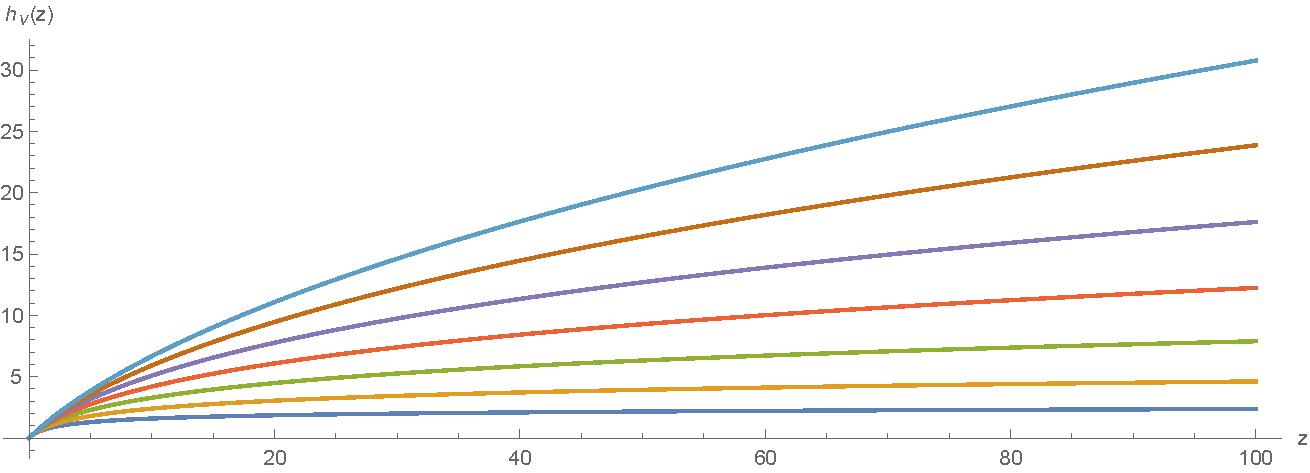
\includegraphics[width=\linewidth]{fig2}
	\end{figure}
	
	先来考虑低温$ T\to 0 $的情况,由\eqref{24a}变形得
	\[\label{25}g_{\frac 32}(z)=\frac{\sqrt 2N}{V}\left(\frac{\pi\hbar^2}{mkT}\right)^{\frac 32}\to+\infty\taghere\]
	所幸$ z\to\infty $的时候$ g_\nu(z)\to\infty $,这保证了\eqref{25}总是有解的,且$ z=\ee^{\mu/kT}\to\infty $. 这里不加证明地给出$ g_\nu(z) $在$ z\to\infty $时的渐进表达式:
	\[\label{26}g_\nu(z)\approx\frac{(\ln z)^\nu}{\Gamma(\nu+1)}+\frac{\pi^2}{6}\frac{(\ln z)^{\nu-2}}{\Gamma(\nu-1)}\quad(z\to\infty)\taghere\]
	\eqref{25}式对每个温度$ T $都唯一确定了化学势$ \mu(T) $. 我们想从\eqref{25}解出$ z $从而解出$ \mu $,为此先把\eqref{26}右侧第一项代入\eqref{25}式中得到
	\[\frac{4(\ln z)^{\frac 32}}{3\sqrt{\pi}}=\frac{\sqrt 2N}{V}\left(\frac{\pi\hbar^2}{mkT}\right)^{\frac 32}\to+\infty\taghere\]
	也就是说
	\[\label{28}\mu(T)=kT\ln z\approx\frac{\hbar^2}{2m}\left(3\pi^2\frac NV\right)^{\frac 23}\taghere\]
	\eqref{28}式是$ T\to 0 $时对$ \mu $的最低阶近似,表明$ T\to 0 $时费米气体的化学势趋于一定值,定义\emph{费米能级}
	\[\label{29}\mu(0):=\frac{\hbar^2}{2m}\left(3\pi^2\frac NV\right)^{\frac 23}\taghere\]
	为$ T=0 $时的化学势。费米能级的概念稍后还会涉及。利用费米能级$ \mu(0) $将\eqref{25}改写为
	\[\label{25'}g_{\frac 32}(z)=\frac{4}{3\sqrt{\pi}}\left(
	\frac{\mu(0)}{kT}\right)^{\frac 32}\tag{\ref{25}$ ' $}\]
	我们继续计算$ \mu $的下一级近似,将\eqref{26}式右边两项均代入\eqref{25'}式得到
	\[\left(\frac{\mu(0)}{kT}\right)^{\frac 32}=\left(\frac{\mu}{kT}\right)^{\frac 32}\left(1+\frac{\pi^2}8\left(\frac{kT}{\mu}\right)^2\right)\]
	也就是说
	\[\label{30}\frac\mu{\mu(0)}=\left(1+\frac{\pi^2}8\left(\frac{kT}{\mu}\right)^2\right)^{-\frac 23}\approx1-\frac{\pi^2}{12}\left(\frac{kT}{\mu(0)}\right)^2\taghere\]
	\eqref{30}式表明低温下化学势$ \mu $随温度上升会下降。
	以及
	\begin{align*}
		g_\nu(z)&\approx\frac 1{\Gamma(\nu+1)}\left(\frac{\mu}{kT}\right)^\nu\left(1+\frac{\pi^2}{6}\nu(\nu-1)\left(\frac{kT}{\mu}\right)^2\right)\\
		&=\frac 1{\Gamma(\nu+1)}\left(\frac{\mu(0)}{kT}\right)^\nu\left(1-\frac{\pi^2}{12}\left(\frac{kT}{\mu(0)}\right)\right)^\nu\left(1+\frac{\pi^2}{6}\nu(\nu-1)\left(\frac{kT}{\mu(0)}\right)^2\right)\\
		&\approx\frac 1{\Gamma(\nu+1)}\left(\frac{\mu(0)}{kT}\right)^\nu\left(1+\frac{\pi^2}{12}(2\nu^2-3\nu)\left(\frac{kT}{\mu(0)}\right)^2\right)\taghere
	\end{align*}
	也就是说
	\begin{align*}
		g_{\frac 32}(z)&=\frac{1}{\Gamma(5/2)}\left(
		\frac{\mu(0)}{kT}\right)^{\frac 32}\\
		g_{\frac 52}(z)&=\frac{1}{\Gamma(7/2)}\left(
		\frac{\mu(0)}{kT}\right)^{\frac 52}\left(1+\frac{5\pi^2}{12}\left(\frac{kT}{\mu(0)}\right)^2\right)
	\end{align*}
	进一步可以算出内能$ U $, 由\eqref{24}式有
	\begin{align*}
	\frac{U}{NkT}&=\frac 32\frac{g_{5/2}(z)}{g_{3/2}(z)}\approx\frac 32\times\frac 25\frac{\mu(0)}{kT}\left(1+\frac{5\pi^2}{12}\left(\frac{kT}{\mu(0)}\right)^2\right)
	\end{align*}
	也就是说
	\[\label{FermiGasEnergy}U=\frac 35N\mu(0)+\frac{\pi^2}{4}\frac{N}{\mu(0)}(kT)^2\taghere\]
	内能\eqref{FermiGasEnergy}右侧第一项为常数,是由于泡利不相容原理带来的内禀能量。第二项正比于$ T^2 $,因此可以得到低温下费米气体热容
	\[C_V=\parDer UT=\frac{\pi^2}{2}Nk\frac{kT}{\mu(0)}\propto T\taghere\]
	
	这里我们不妨从另一个角度重新思考简并费米气体在低温下的性质:为什么低温下内能\eqref{FermiGasEnergy}是一个常数项加一个$ T^2 $项呢?
	
	我们知道费米子服从泡利不相容原理。在$ T=0\unit{K} $时没有热涨落,费米子首先填入最低能级,在最低能级占满后填入次低能级,依次填满低能级直到所有费米子都填进某个能级里。这一过程就好像拿着一袋苹果上楼,每上一层楼就在这一层留下两个苹果直到袋子里苹果用完。因此$ T=0\unit{K} $时的费米分布\eqref{FermiDistribution}应该存在某个临界能量$ \mu(0) $, 低于$ \mu(0) $的能级完全填满,而高于$ \mu(0) $的能级完全空着,也就是说
	\[f^0_{\text{Fermi}}(E)=\begin{cases}
	1,&E\le\mu(0)\\0,&E>\mu(0)
	\end{cases}\taghere\]
	费米能级$ \mu(0) $仍由\eqref{3a}确定:
	\[N=\int_0^{\mu(0)}g(E)\diff E=\frac{\sqrt{2}m^{\frac 32}V}{\pi^2\hbar^3}\times\frac 23\left(\mu(0)\right)^{\frac 23}\taghere\]
	即
	\[\mu(0)=\frac{\hbar^2}{2m}\left(3\pi^2\frac NV\right)^{\frac 23}\tag{\ref{29}$ ' $}\]
	这时候的费米气体内能
	\[U=\int_0^{\mu(0)}Eg(E)\diff E=\frac 35N\mu(0)\taghere\]
	而当$ T>0 $但仍然属于低温范围内的时候,我们可以把费米分布$ f_{\text{Fermi}}(E) $画出来看看是什么样的:
	
	\begin{multicols}{2}
		\noindent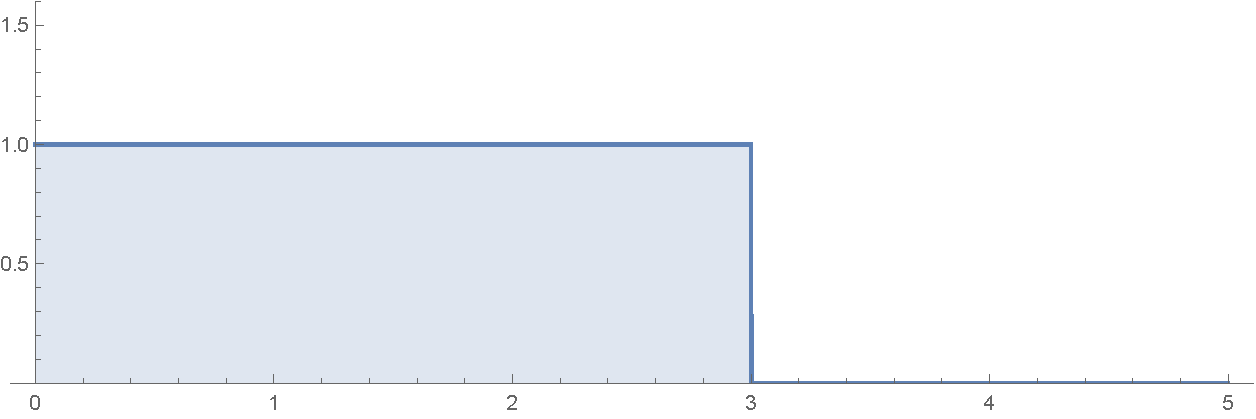
\includegraphics[width=\linewidth]{fig3L}
		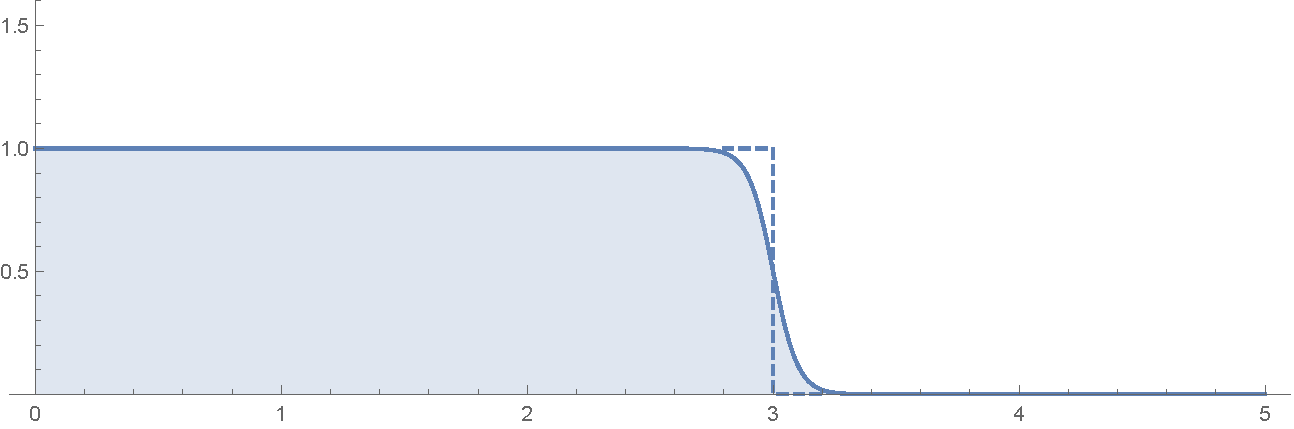
\includegraphics[width=\linewidth]{fig3R}
	\end{multicols}

	上图左侧代表$ T=0\unit{K} $时的费米分布,而右侧代表$ T>0 $,可以看到部分$ \mu(0) $以下的费米子被激发到了$ \mu(0) $以上的能级。但是在低温下这种激发非常微弱,只涉及到了$ \mu(0) $附近能级内的费米子,只有这部分费米子对低温下的气体内能变化以及热容有贡献,因此我们考虑$ \mu(0)\pm2kT $范围内的能级:
	\begin{align*}
	U&\approx\int_{\mu(0)-2kT}^{\mu(0)+2kT}Eg(E)\left(f(E)-f^0(E)\right)\diff E\\
	&\approx\int_{\mu(0)-2kT}^{\mu(0)+2kT}\frac{Eg(E)\diff E}{\ee^{\frac{E-\mu(0)}{kT}}+1}-\int_{\mu(0)-2kT}^{\mu(0)}Eg(E)\diff E\\
	&\approx \frac{\sqrt{2}m^{\frac 32}V}{\pi^2\hbar^3}kT\left(\int_{0}^{2}\frac{(\mu(0)-kTx)^{\frac 32}\ee^x}{\ee^x+1}\diff x+\int_0^2\frac{(\mu(0)+kTx)^{\frac 32}}{\ee^x+1}\diff x-\int_0^2(\mu(0)-kTx)^{\frac 32}\diff x\right)\\
	&=\frac{\sqrt{2}m^{\frac 32}V}{\pi^2\hbar^3}kT\int_0^2\frac{(\mu(0)+kTx)^{\frac 32}-(\mu(0)-kTx)^{\frac 32}}{\ee^x+1}\diff x\\
	&\approx\frac{\sqrt{2}m^{\frac 32}V}{\pi^2\hbar^3}kT(\mu(0))^{\frac 32}\int_0^2\frac{1}{\ee^x+1}\cdot\frac{3kTx}{\mu(0)}\diff x
	\end{align*}
	总之
	\[U=\frac 92\frac{N}{\mu(0)}(kT)^2\int_0^2\frac{x\diff x}{\ee^x+1}\approx1.97\frac{N(kT)^2}{\mu(0)}\taghere\]
	式\eqref{FermiGasEnergy}给出$ U\approx2.47N(kT)^2/\mu(0) $. 系数算的不太准,但是至少还是得出了内能$ U\propto T^2 $的结论,再一次说明了$ C_V\propto T $.
	
	
	金属中的自由电子气就是常见的费米气体。电子热容$ C_V^{\text{electron}} $和晶格热容$ C_V^{\text{lattice}} $对金属的热容均有贡献。固体物理会提到在低温下这两个热容的特点是
	\[C_V^{\text{electron}}\propto T\,,\quad C_V^{\text{lattice}}\propto T^3\]
	因此在极低的温度下金属热容主要来源于电子热容。下图展示了一个典型的金属热容实验测量值\footnote{引用自黄昆《固体物理学》\emph{金属电子论}章节}。
	\begin{figure}[h]
		\centering
		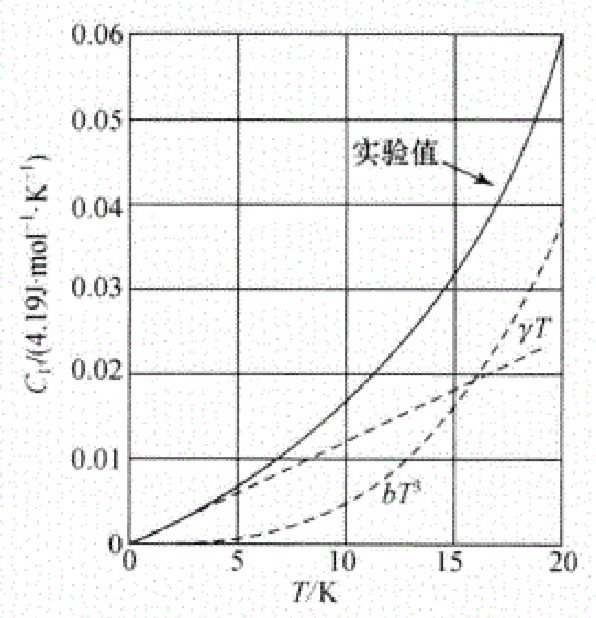
\includegraphics[width=.5\linewidth]{MetalCapacity}
	\end{figure}
	
	在常温下费米气体的简并效应同样被经典性掩盖,式\eqref{24}给出
	\[\label{38}\frac{U}{NkT}=\frac 32\frac{g_{5/2}(z)}{g_{3/2}(z)}\taghere\]
	在$ kT\gg\mu(0)  $的时候$ g_\nu(z)\to 0 $. 那么由\eqref{25'}式有
	\[z\approx g_{\frac 32}(z)=\frac{4}{3\sqrt{\pi}}\left(\frac{\mu(0)}{kT}\right)^{\frac 32}\]
	$ g_\nu(z)=-h_\nu(-z) $, 在$ 0\le zle 1 $的时候有
	\[\label{39}g_\nu(z)=\sum_{n=1}^{\infty}\frac{(-1)^{n+1}z^n}{n^\nu}\approx z-\frac{z}{2^\nu}\taghere\]
	将\eqref{39}式代入\eqref{38}式中有
	\begin{align*}
	\frac{U}{NkT}&\approx\frac 32\cdot\frac{1-\dfrac{z}{2^{5/2}}}{1-\dfrac{z}{2^{3/2}}}\approx\frac 32\left(1+\frac{1}{4\sqrt{2}}\times\frac{4}{3\sqrt{\pi}}\left(\frac{\mu(0)}{kT}\right)^{\frac 32}\right)
	\end{align*}
	即\[U\approx\frac 32NkT\left(1+\frac{1}{3\sqrt{2\pi}}\left(\frac{\mu(0)}{kT}\right)^{\frac 32}\right)\approx\frac 32NkT\taghere\]
	\newpage
	\section{总结}
	总的来说,玻色气体和费米气体由于量子特性,在低温下进入简并态,并且具有不同的热容特性。
	
	对于玻色气体来说,由于玻色子之间的全同性,在低于临界温度$ T_C $的时候会有大量的玻色子被“冻结”在能量为0的基态,数量$ N_{=0} $为
	\[N_{=0}=N\left(1-\left(\frac{T}{T_C}\right)^2\right)\taghere\]
	剩下的玻色子处于激发态,为玻色气体提供了内能
	\[U=\frac{3\zeta(5/2)}{2\zeta(3/2)}NkT\left(\frac{T}{T_C}\right)^{\frac 32}\approx0.770NkT\left(\frac{T}{T_C}\right)^{\frac 32}\taghere\]
	热容$ C_V\propto T^{3/2} $:
	\[C_V=\frac{5U}{2T}\approx1.925Nk\left(\frac{T}{T_C}\right)^{\frac 32}\taghere\]
	
	对于费米气体来说,由于泡利不相容原理,在$ T=0 $时费米子必须依次填满能量较低的能级,直到费米能级$ \mu(0) $为止。低温$ T>0 $时只有费米能级$ \mu(0) $附近的费米子能被激发。低温费米气体有内能
	\[U=\frac 35N\mu(0)+\frac{\pi^2}{4}\frac{N}{\mu(0)}(kT)^2\taghere\]
	上式第一项代表了$ T=0 $时能级范围$ 0 $至$ \mu(0) $上所有态均被填满具有的内能,第二项代表能量接近$ \mu(0) $的费米子被激发所带来的内能。对应费米气体的低温热容$ C_V\propto T $:
	\[C_V=\frac{\pi^2}{2}\frac{kT}{\mu(0)}Nk\taghere\]
	
	而在常温下玻色气体和费米气体共同退化至经典情形
	\[U\approx\frac 32NkT\,,\,C_V\approx\frac 32Nk\taghere\]
\end{document}